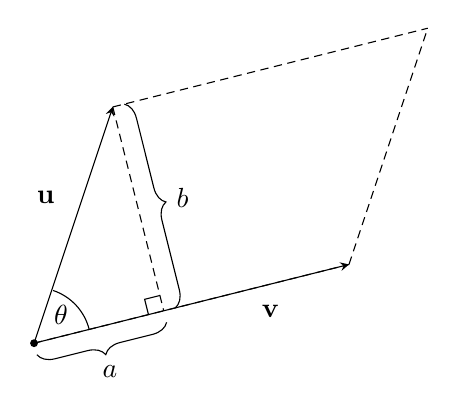
\begin{tikzpicture}
    \coordinate (a) at (0,0);
    \coordinate (b) at (1,3);
    \coordinate (c) at (4,1);
    \coordinate (d) at (1.6470,0.41176);
    \coordinate (e) at (1.4530,0.3633);
    \coordinate (f) at (1.4045,0.5573);
    \coordinate (g) at (1.5985,0.6058);
    \coordinate (h) at (5,4);
    \fill (a) circle (0.05);
    % \fill (e) circle (0.05);
    % \fill (f) circle (0.05);
    % \fill (g) circle (0.05);
    \draw[-stealth] (a)--(b) node[midway, xshift=-10pt, yshift=10pt] {$\textbf{u}$};
    \draw[-stealth] (a)--(c) node[pos=0.75, yshift=-10pt] {$\textbf{v}$};
    \draw[densely dashed] (b)--(h);
    \draw[densely dashed] (c)--(h);
    % \node at (-.3,-.3) {$(0,0)$};
    % \node at (4.2,3.2) {$B$};
    \draw[densely dashed] (a)--(c);
    \draw[densely dashed] (b)--(d);
    % \draw (c) rectangle (3.8,0.2);
    \draw (e) -- (f) -- (g);
    \draw (0.7,0.175) arc (14.036:71.565:0.7) node[midway, xshift=-5.5pt, yshift=-3.5pt] {$\theta$};
    \draw [decorate,decoration={brace,amplitude=6pt,mirror,raise=1ex}] (a) -- (d) node[midway,xshift=4pt,yshift=-16pt]{$a$};
    \draw [decorate,decoration={brace,amplitude=6pt,mirror,raise=1ex}] (d) -- (b) node[midway,xshift=16pt,yshift=4pt]{$b$};
\end{tikzpicture}